\documentclass[12pt,a4paper]{article}

% ── Packages ──
\usepackage[margin=1in]{geometry}
\usepackage{graphicx}
\usepackage{listings}
\usepackage{xcolor}
\usepackage{hyperref}
\usepackage{booktabs}
\usepackage{float}
\usepackage{caption}
\usepackage{subcaption}
\usepackage{amsmath}
\usepackage{fancyhdr}
\usepackage{titlesec}
\usepackage{enumitem}
\graphicspath{{report_assets/}}

% ── Colors ──
\definecolor{codeblue}{RGB}{0,102,204}
\definecolor{codegray}{RGB}{128,128,128}
\definecolor{codegreen}{RGB}{0,128,0}
\definecolor{codebg}{RGB}{245,245,245}
\definecolor{linkblue}{RGB}{0,80,160}

% ── Hyperlinks ──
\hypersetup{
    colorlinks=true,
    linkcolor=linkblue,
    urlcolor=linkblue,
    citecolor=linkblue
}

% ── Code Listing Style ──
\lstdefinestyle{gostyle}{
    language=Go,
    backgroundcolor=\color{codebg},
    basicstyle=\ttfamily\footnotesize,
    keywordstyle=\color{codeblue}\bfseries,
    commentstyle=\color{codegreen}\itshape,
    stringstyle=\color{red!70!black},
    numberstyle=\tiny\color{codegray},
    numbers=left,
    numbersep=8pt,
    frame=single,
    framerule=0.5pt,
    rulecolor=\color{codegray!50},
    breaklines=true,
    breakatwhitespace=true,
    tabsize=4,
    showstringspaces=false,
    captionpos=b,
    xleftmargin=2em,
    framexleftmargin=1.5em
}

\lstdefinestyle{pythonstyle}{
    language=Python,
    backgroundcolor=\color{codebg},
    basicstyle=\ttfamily\footnotesize,
    keywordstyle=\color{codeblue}\bfseries,
    commentstyle=\color{codegreen}\itshape,
    stringstyle=\color{red!70!black},
    numberstyle=\tiny\color{codegray},
    numbers=left,
    numbersep=8pt,
    frame=single,
    framerule=0.5pt,
    rulecolor=\color{codegray!50},
    breaklines=true,
    tabsize=4,
    showstringspaces=false,
    captionpos=b,
    xleftmargin=2em,
    framexleftmargin=1.5em
}

\lstdefinestyle{csvstyle}{
    backgroundcolor=\color{codebg},
    basicstyle=\ttfamily\footnotesize,
    frame=single,
    framerule=0.5pt,
    rulecolor=\color{codegray!50},
    breaklines=true,
    captionpos=b,
    xleftmargin=2em,
    framexleftmargin=1.5em
}

\lstdefinestyle{jsonstyle}{
    backgroundcolor=\color{codebg},
    basicstyle=\ttfamily\footnotesize,
    frame=single,
    framerule=0.5pt,
    rulecolor=\color{codegray!50},
    breaklines=true,
    captionpos=b,
    xleftmargin=2em,
    framexleftmargin=1.5em,
    stringstyle=\color{red!70!black},
    keywordstyle=\color{codeblue}
}

% ── Header/Footer ──
\pagestyle{fancy}
\setlength{\headheight}{15pt}
\fancyhf{}
\fancyhead[L]{\small Lab 5: Load Balanced Back-end}
\fancyhead[R]{\small Sneha Nagmoti}
\fancyfoot[C]{\thepage}
\renewcommand{\headrulewidth}{0.4pt}

% ── Section formatting ──
\titleformat{\section}{\large\bfseries}{\thesection.}{0.5em}{}
\titleformat{\subsection}{\normalsize\bfseries}{\thesubsection.}{0.5em}{}

% ══════════════════════════════════════════════════════════════
\begin{document}

% ── Title Page ──
\begin{titlepage}
\centering
\vspace*{2cm}

{\LARGE\bfseries Lab 5: Load Balanced Back-end\par}
\vspace{0.5cm}
\vspace{2cm}

\begin{tabular}{rl}
    \textbf{Student Name:} & Sneha Nagmoti \\[6pt]
    \textbf{Roll Number:}  & 12342090 \\[6pt]
    \textbf{Date:}         & August 24, 2026 \\[6pt]
    \textbf{Course:}       & CS559: Computer Systems Design \\[6pt]
    \textbf{GitHub Repo:}  & \url{https://github.com/snehanagmoti/group-chat-app} \\[6pt]
    \textbf{Branch:}       & \texttt{sneha} \\[6pt]
    \textbf{Live Demo:}    & \url{https://10.1.75.53:3237/} \\
\end{tabular}

\vspace{1cm}
\textit{The canonical load-balancer source used for this report is reproduced in the appendix. The project repository and intended submission branch are linked above.}

\vspace{1cm}

\begin{tabular}{|l|l|l|l|}
\hline
\textbf{System} & \textbf{Role} & \textbf{SSH Port} & \textbf{Internal IP} \\
\hline
stu70\_sys1 & Load Balancer   & 2237 & 172.17.0.38 \\
stu70\_sys2 & Backend-1       & 2238 & 172.17.0.39 \\
stu70\_sys3 & Backend-2       & 2239 & 172.17.0.40 \\
stu70\_sys4 & Backend-3       & 2240 & 172.17.0.41 \\
\hline
\end{tabular}

\vspace{0.5cm}
{\small SSH Host: \texttt{10.1.75.53} \quad|\quad Username: \texttt{student}}

\vspace{0.35cm}
{\small Application mappings: UI \texttt{3000 $\to$ 3237}; load balancer \texttt{4000 $\to$ 4237}; backends \texttt{5000 $\to$ 5238/5239/5240}.}

\vfill
\end{titlepage}

% ── Table of Contents ──
\tableofcontents
\newpage

% ══════════════════════════════════════════════════════════════
\section{Introduction}

This report documents the implementation and evaluation of a \textbf{load-balanced back-end} system for Lab~5. The objective is to distribute incoming HTTP requests across multiple back-end servers using a custom load balancer, and to measure and compare performance metrics under different configurations.

\subsection{Objectives}
\begin{enumerate}[leftmargin=2em]
    \item Implement a reverse-proxy load balancer in Go on Sys1.
    \item Deploy the messaging application back-end (from the previous assignment) on Sys2, Sys3, and Sys4.
    \item Build a concurrent load generator to stress-test the system.
    \item Measure performance with a single back-end (Sys2 only).
    \item Measure performance with all three back-ends (Sys2, Sys3, Sys4).
    \item Compare results and analyze the benefits of load balancing.
\end{enumerate}

% ══════════════════════════════════════════════════════════════
\section{System Architecture}

\subsection{Overview}

The system consists of four components deployed across four machines:

\begin{figure}[H]
\centering
\fbox{\parbox{0.85\textwidth}{\centering
\vspace{0.5cm}
\texttt{Load Generator} $\xrightarrow{\text{HTTP}}$
\texttt{Sys1 (Load Balancer :4000)} $\xrightarrow{\text{Round-Robin}}$
$\begin{cases}
\texttt{Sys2 (Backend-1 :5000)} \\
\texttt{Sys3 (Backend-2 :5000)} \\
\texttt{Sys4 (Backend-3 :5000)}
\end{cases}$
\vspace{0.5cm}
}}
\caption{System architecture: Load Generator $\to$ Load Balancer $\to$ Back-ends}
\label{fig:architecture}
\end{figure}

\begin{figure}[H]
\centering
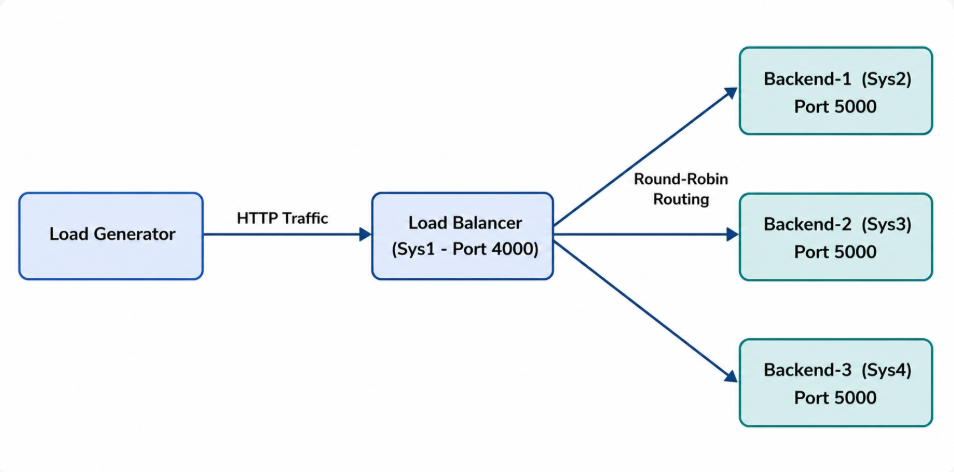
\includegraphics[width=0.85\textwidth]{p1.png}
\caption{System architecture overview}
\label{fig:arch-screenshot}
\end{figure}

\subsection{Assigned Systems}

\begin{table}[H]
\centering
\caption{Assigned system details}
\label{tab:systems}
\small
\begin{tabular}{lllll}
\toprule
\textbf{System} & \textbf{Role} & \textbf{SSH Command} & \textbf{Internal IP} & \textbf{Service Port} \\
\midrule
stu70\_sys1 & Load Balancer & \texttt{10.1.75.53:2237} & 172.17.0.38 & \texttt{4000 $\to$ 4237} \\
stu70\_sys2 & Backend-1     & \texttt{10.1.75.53:2238} & 172.17.0.39 & \texttt{5000 $\to$ 5238} \\
stu70\_sys3 & Backend-2     & \texttt{10.1.75.53:2239} & 172.17.0.40 & \texttt{5000 $\to$ 5239} \\
stu70\_sys4 & Backend-3     & \texttt{10.1.75.53:2240} & 172.17.0.41 & \texttt{5000 $\to$ 5240} \\
\bottomrule
\end{tabular}
\end{table}

% ══════════════════════════════════════════════════════════════
\section{Implementation}

\subsection{Load Balancer (\texttt{cmd/load-balancer} and \texttt{internal/loadbalancer})}

The load balancer is implemented in Go. The command entry point is
\texttt{cmd/load-balancer/main.go}; the canonical implementation is
\texttt{internal/loadbalancer/loadbalancer.go}. It provides:

\begin{itemize}[leftmargin=2em]
    \item \textbf{Health-aware round robin} for new requests, skipping unhealthy replicas.
    \item \textbf{Cookie affinity} for stateful messaging sessions while preserving round robin for new clients.
    \item \textbf{HTTPS/WSS reverse proxying} through \texttt{httputil.NewSingleHostReverseProxy}.
    \item \textbf{Concurrent active health checks} against each backend's \texttt{/health} endpoint.
    \item \textbf{Configurable connection, TLS, response-header, and total request timeouts}.
    \item \textbf{Monitoring endpoints} at \texttt{/lb/health}, \texttt{/lb/status}, and \texttt{/lb/metrics}.
    \item \textbf{Thread-safe metrics} for totals, failures, backend errors, in-flight requests, and latency percentiles.
    \item \textbf{WebSocket-safe response recording}, including flush and connection hijacking support.
\end{itemize}

\subsubsection{Backend and Metrics State}

Atomic fields protect backend liveness, in-flight counts, and request counters. A bounded, mutex-protected latency tracker calculates average, p50, p95, and p99 latency without unbounded memory growth.

\begin{lstlisting}[style=gostyle, caption={Core backend and load-balancer state}]
type Backend struct {
    ID       int
    URL      *url.URL
    Alive    atomic.Bool
    InFlight atomic.Int64
}

type LoadBalancer struct {
    backends       []*Backend
    next           atomic.Uint64
    metrics        *Metrics
    transport      *http.Transport
    healthClient   *http.Client
    backendTimeout time.Duration
    affinity       bool
}
\end{lstlisting}

\subsubsection{Round-Robin and Affinity Selection}

For a client with a valid \texttt{pixelchat\_backend} cookie, the balancer reuses that healthy replica so room and WebSocket state remain consistent. Otherwise, an atomic compare-and-swap counter selects the next healthy backend. Verification produced an exact 4/4/4 split for twelve cookie-free requests, a 6/6 split after one backend was stopped, and 4/4/4 again after recovery.

\subsubsection{Health Checks and Timeouts}

\texttt{checkAllBackends} probes the replicas concurrently. The health loop runs once per second, uses a two-second health timeout, consumes and closes response bodies, and updates each backend's atomic \texttt{Alive} flag. The shared transport uses a two-second dial/TLS-handshake timeout, a three-second backend response timeout, connection pooling, and TLS~1.2 or newer. Self-signed backend certificates are accepted only through the explicit lab-only flag \texttt{-backend-insecure-skip-verify}.

\subsubsection{Reverse Proxy, WebSockets, and Error Handling}

HTTP requests and \texttt{/ws} upgrades use the same reverse proxy. A custom status recorder implements \texttt{Flush}, \texttt{Hijack}, \texttt{Push}, and \texttt{ReadFrom}, so WebSocket upgrades remain valid. A genuine backend error marks that replica unhealthy; a downstream client cancellation does not incorrectly eject a healthy backend. The selected backend is exposed in \texttt{X-Load-Balancer-Backend} for verification.

\subsubsection{Monitoring Endpoints}

\begin{table}[H]
\centering
\caption{Load Balancer monitoring endpoints}
\label{tab:endpoints}
\begin{tabular}{ll}
\toprule
\textbf{Endpoint} & \textbf{Purpose} \\
\midrule
\texttt{/lb/health}  & Confirm that the load balancer is alive \\
\texttt{/lb/status}  & Return backend URLs, health, and in-flight counts (JSON) \\
\texttt{/lb/metrics} & Return request counters and latency statistics (JSON) \\
\texttt{/}           & Forward HTTP or WebSocket traffic to a healthy backend \\
\bottomrule
\end{tabular}
\end{table}

\begin{figure}[H]
\centering
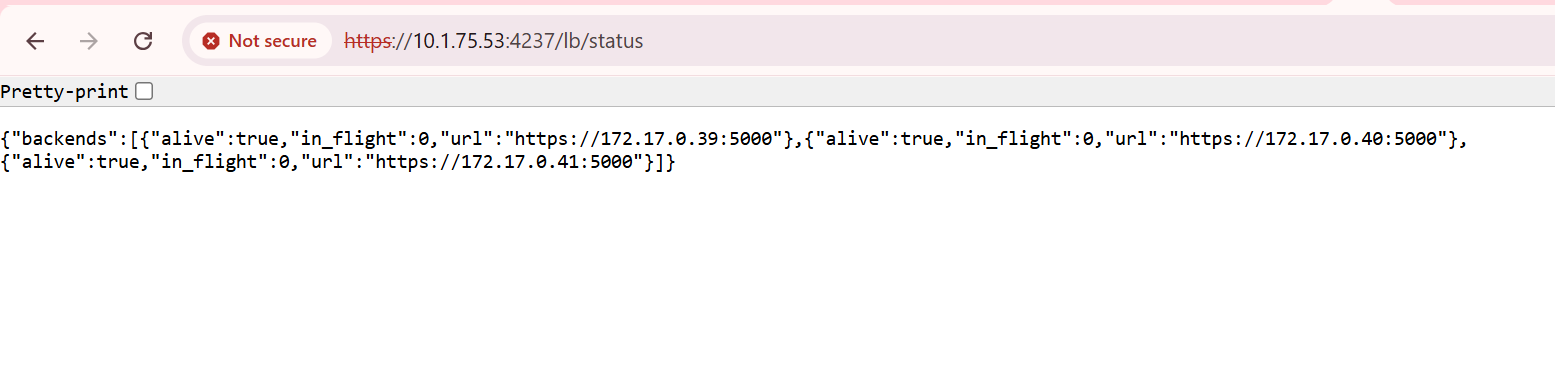
\includegraphics[width=0.85\textwidth]{p2.png}
\caption{Load Balancer \texttt{/lb/status} endpoint showing healthy backends}
\label{fig:lb-status}
\end{figure}

% ──────────────────────────────────────────────────────────────
\subsection{Back-end Server (\texttt{server/server.py})}

The back-end is the \textbf{FastAPI WebSocket messaging application} from the previous assignment, extended with:

\begin{itemize}[leftmargin=2em]
    \item \textbf{\texttt{/health} endpoint} --- returns \texttt{\{"status": "ok"\}} for load balancer health checks.
    \item \textbf{Delay simulation} --- \texttt{/?delay=100ms} adds artificial processing delay using \texttt{asyncio.sleep()}.
    \item \textbf{Failure simulation} --- \texttt{/?fail=true} returns HTTP 503.
    \item \textbf{Backend identification} --- adds response headers that reveal which replica handled a request.
    \item \textbf{Configurable port} --- via the \texttt{PORT} environment variable (set to 5000).
\end{itemize}

\begin{lstlisting}[style=pythonstyle, caption={Health check endpoint added to the messaging server}]
@app.get("/health")
async def health_check():
    """Health check endpoint for the Load Balancer."""
    return {"status": "ok"}
\end{lstlisting}

\begin{figure}[H]
\centering
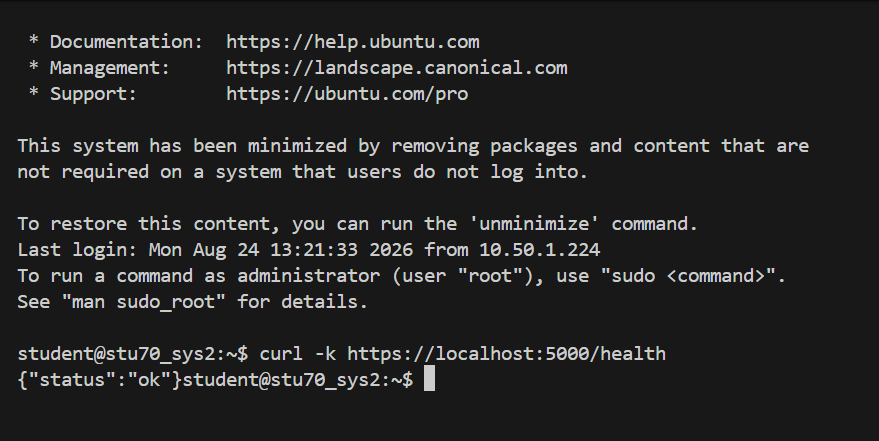
\includegraphics[width=0.85\textwidth]{p3.png}
\caption{Backend health check response}
\label{fig:backend-health}
\end{figure}

% ──────────────────────────────────────────────────────────────
\subsection{Load Generator (\texttt{cmd/load-generator} and \texttt{internal/loadgenerator})}

The load generator is a concurrent HTTP client written in Go that uses a worker pool pattern:

\begin{itemize}[leftmargin=2em]
    \item Accepts command-line flags: \texttt{-url}, \texttt{-requests}, \texttt{-concurrency}, \texttt{-timeout}, \texttt{-experiment}, \texttt{-out}, \texttt{-csv}
    \item Creates $N$ concurrent goroutine workers consuming from a shared job channel
    \item Records per-request latency for every attempted request
    \item Calculates: throughput (RPS), dropout percentage, p50/p95/p99 latency percentiles
    \item Supports self-signed lab TLS through the explicit \texttt{-insecure} flag
    \item Outputs results as JSON (per experiment) and CSV (cumulative)
\end{itemize}

\subsubsection{Metrics Formulas}

\begin{align}
\text{Throughput (RPS)} &= \frac{\text{Successful Requests}}{\text{Elapsed Time (seconds)}} \\[8pt]
\text{Dropout (\%)} &= \frac{\text{Failed Requests}}{\text{Total Requests}} \times 100 \\[8pt]
\text{p}N &= \text{Latency at index } \lfloor \text{len(sorted\_latencies)} \times \frac{N}{100} \rfloor
\end{align}

\begin{lstlisting}[style=gostyle, caption={Worker pool pattern in the load generator}]
for i := 0; i < concurrency; i++ {
    wg.Add(1)
    go func() {
        defer wg.Done()
        client := &http.Client{Timeout: timeout}
        for range jobs {
            reqStart := time.Now()
            resp, err := client.Do(req)
            if err != nil {
                failCount.Add(1)
                continue
            }
            io.Copy(io.Discard, resp.Body)
            resp.Body.Close()
            if resp.StatusCode == http.StatusOK {
                successCount.Add(1)
                latencies <- time.Since(reqStart)
            } else {
                failCount.Add(1)
            }
        }
    }()
}
\end{lstlisting}

% ══════════════════════════════════════════════════════════════
\section{Deployment}

\subsection{Backend Deployment (Sys2, Sys3, Sys4)}

The messaging application server was deployed to all three backend systems using an automated Python script (\texttt{deploy\_and\_run.py}):

\begin{enumerate}[leftmargin=2em]
    \item SSH into each system (ports 2238, 2239, 2240)
    \item Upload the FastAPI server, database helper, environment file, TLS certificate/key, and required client assets
    \item Install dependencies: \texttt{pip3 install fastapi uvicorn websockets python-multipart bcrypt cryptography python-dotenv}
    \item Start the server on port 5000 (HTTPS): \texttt{PORT=5000 python3 server/server.py}
    \item Verify health: \texttt{curl -k https://127.0.0.1:5000/health}
\end{enumerate}

\subsection{Load Balancer Deployment (Sys1)}

\begin{enumerate}[leftmargin=2em]
    \item Upload the Go module and build: \texttt{go build -o load\_balancer ./cmd/load-balancer}
    \item Start with backend URLs:
\begin{lstlisting}[style=csvstyle]
./load_balancer \
  -backends https://172.17.0.39:5000,https://172.17.0.40:5000,https://172.17.0.41:5000 \
  -port 4000 -backend-insecure-skip-verify \
  -tls-cert cert.pem -tls-key key.pem
\end{lstlisting}
    \item Verify: \texttt{curl -k https://127.0.0.1:4000/lb/health}
\end{enumerate}

\begin{figure}[H]
\centering
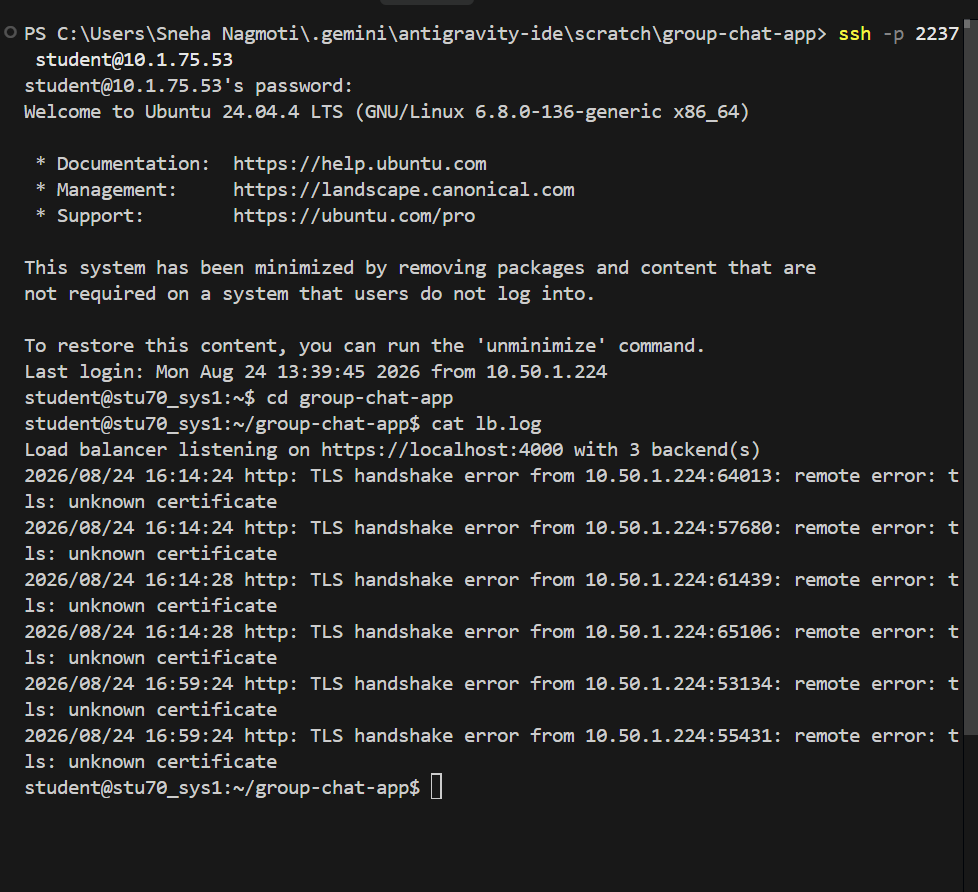
\includegraphics[width=0.85\textwidth]{p4.png}
\caption{Load Balancer startup on Sys1}
\label{fig:lb-startup}
\end{figure}

The first line in Figure~\ref{fig:lb-startup} confirms the HTTPS listener on port~4000 with three backends. The later ``unknown certificate'' handshake messages were produced by clients that had not yet trusted the self-signed lab certificate; they do not indicate a load-balancer or backend failure.

% ══════════════════════════════════════════════════════════════
\section{Experiments}

\subsection{Experiment Parameters}

Both experiments used identical parameters to ensure a fair comparison:

\begin{table}[H]
\centering
\caption{Experiment configuration}
\label{tab:params}
\begin{tabular}{ll}
\toprule
\textbf{Parameter} & \textbf{Value} \\
\midrule
Total Requests      & 5,000 \\
Concurrency         & 200 workers \\
Simulated Delay     & 100ms per request (\texttt{?delay=100ms}) \\
Client Timeout      & 3 seconds \\
Backend Timeout (LB)& 3 seconds \\
Health Check Interval & 1 second \\
Traffic Source       & Local workstation \\
Target               & \texttt{https://10.1.75.53:4237} \\
\bottomrule
\end{tabular}
\end{table}

The simulated delay (\texttt{?delay=100ms}) models realistic backend processing time (e.g., database queries or computation). High concurrency (200 workers) creates contention that reveals the benefit of distributing work. For the assignment measurement, the Go load-generator binary ran on the local Windows workstation and sent traffic through Sys1's public mapped port~4237. The automation changed only the Sys1 backend list over SSH; it did not move the generator onto Sys1.

% ──────────────────────────────────────────────────────────────
\subsection{Experiment 1: Single Backend}

\textbf{Configuration:} Load Balancer $\to$ Sys2 only

\begin{lstlisting}[style=csvstyle, caption={Experiment 1 --- LB with single backend}]
# Sys1: one-backend load-balancer configuration
./load_balancer -backends https://172.17.0.39:5000 \
    -port 4000 -backend-insecure-skip-verify \
    -tls-cert cert.pem -tls-key key.pem

# Local workstation
tmp/bin/load_generator.exe \
    -url 'https://10.1.75.53:4237/?delay=100ms' \
    -requests 5000 -concurrency 200 -timeout 3s \
    -experiment 1_backend -out 1_backend.json \
    -csv results.csv -insecure
\end{lstlisting}

\textbf{LB Status:}
\begin{lstlisting}[style=jsonstyle]
{"backends":[{"url":"https://172.17.0.39:5000","alive":true,"in_flight":0}]}
\end{lstlisting}

Sys1's \texttt{/lb/metrics} endpoint recorded 5,000 forwarded requests. The final client-observed values are reported consistently in Section~\ref{sec:results}.

\begin{figure}[H]
\centering
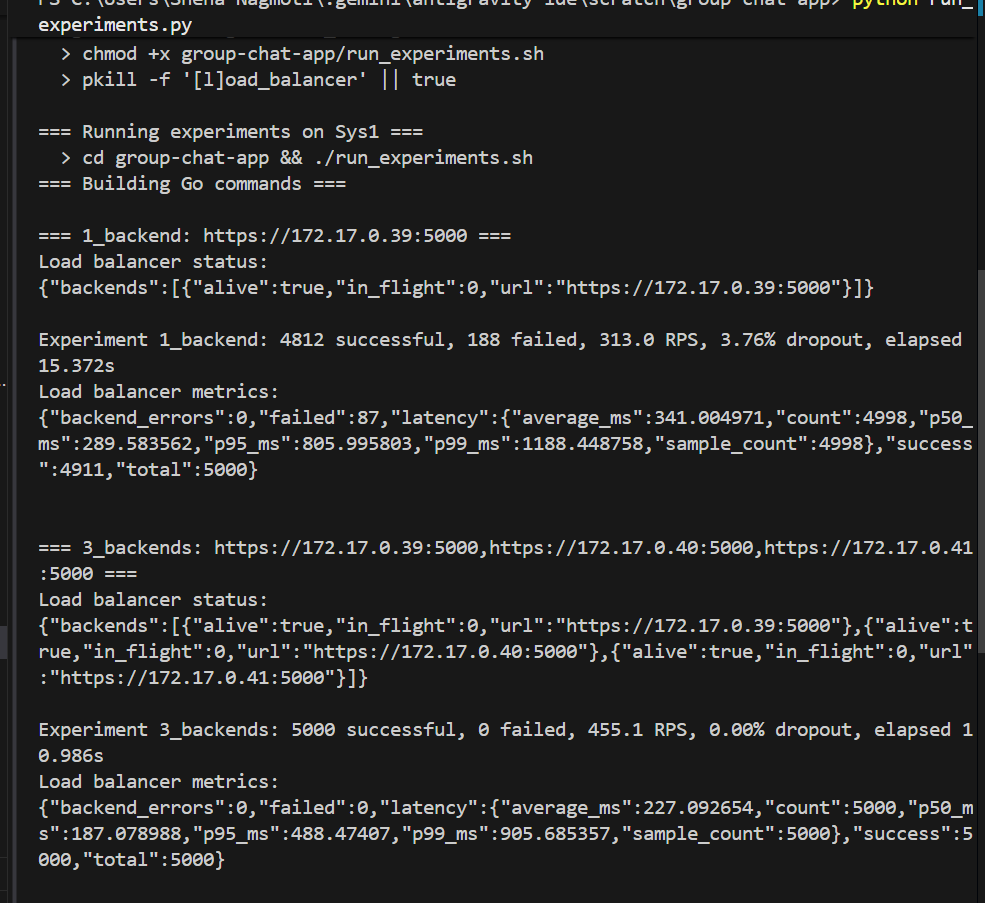
\includegraphics[width=0.85\textwidth]{p5.png}
\caption{Experiment 1: Single backend test execution}
\label{fig:exp1-run}
\end{figure}

Figure~\ref{fig:exp1-run} is retained in its original experiment context as an initial deployment sanity run executed on Sys1. Its terminal values are not mixed with the final local-workstation dataset used in the comparison table.

% ──────────────────────────────────────────────────────────────
\subsection{Experiment 2: Three Backends}

\textbf{Configuration:} Load Balancer $\to$ Sys2 + Sys3 + Sys4

\begin{lstlisting}[style=csvstyle, caption={Experiment 2 --- LB with three backends}]
# Sys1: normal three-backend configuration
./load_balancer \
    -backends https://172.17.0.39:5000,https://172.17.0.40:5000,https://172.17.0.41:5000 \
    -port 4000 -backend-insecure-skip-verify \
    -tls-cert cert.pem -tls-key key.pem

# Local workstation
tmp/bin/load_generator.exe \
    -url 'https://10.1.75.53:4237/?delay=100ms' \
    -requests 5000 -concurrency 200 -timeout 3s \
    -experiment 3_backends -out 3_backends.json \
    -csv results.csv -insecure
\end{lstlisting}

\textbf{LB Status:}
\begin{lstlisting}[style=jsonstyle]
{"backends":[
  {"url":"https://172.17.0.39:5000","alive":true,"in_flight":0},
  {"url":"https://172.17.0.40:5000","alive":true,"in_flight":0},
  {"url":"https://172.17.0.41:5000","alive":true,"in_flight":0}
]}
\end{lstlisting}

Sys1's \texttt{/lb/metrics} endpoint again recorded 5,000 forwarded requests, with all three replicas healthy after the run.

\begin{figure}[H]
\centering
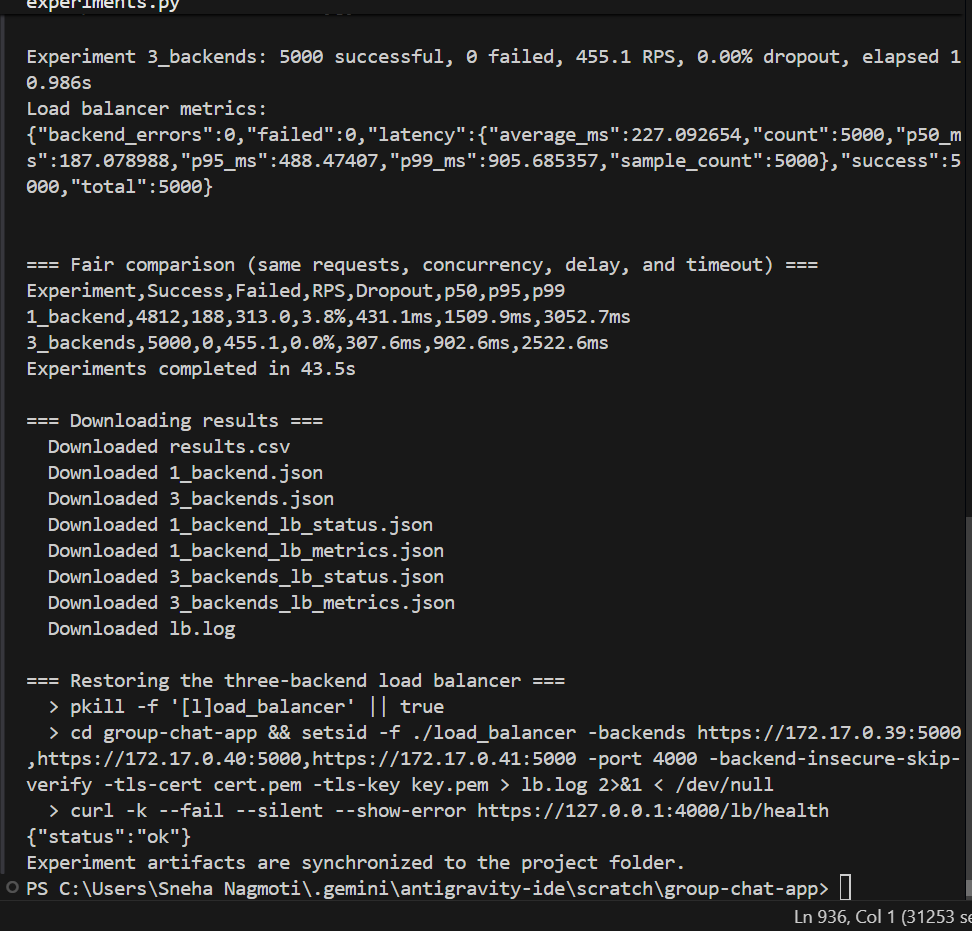
\includegraphics[width=0.85\textwidth]{p6.png}
\caption{Experiment 2: Three backend test execution}
\label{fig:exp2-run}
\end{figure}

Figure~\ref{fig:exp2-run} is the corresponding initial three-backend sanity run. The screenshot remains in the same experiment section; the final comparison below uses the later controlled local-workstation run for both configurations.

% ══════════════════════════════════════════════════════════════
\section{Results and Comparison}
\label{sec:results}

\subsection{Raw Results (results.csv)}

\begin{lstlisting}[style=csvstyle, caption={Generated results.csv}]
Experiment,Success,Failed,RPS,Dropout,p50,p95,p99
1_backend,5000,0,339.4,0.0%,416.4ms,1291.8ms,3466.2ms
3_backends,4999,1,439.6,0.02%,300.2ms,828.1ms,3980.4ms
\end{lstlisting}

\subsection{Comparison Table}

\begin{table}[H]
\centering
\caption{Performance comparison: 1 Backend vs.\ 3 Backends}
\label{tab:comparison}
\begin{tabular}{lrrr}
\toprule
\textbf{Metric} & \textbf{1 Backend} & \textbf{3 Backends} & \textbf{Improvement} \\
\midrule
Successful Requests & 5,000        & 4,999        & $-1$ request \\
Failed Requests     & 0            & 1            & $+1$ request \\
Throughput (RPS)    & 339.4        & 439.6        & +29.5\% \\
Dropout (\%)        & 0.00\%       & 0.02\%       & +0.02 pp \\
p50 Latency         & 416 ms       & 300 ms       & $-$27.9\% \\
p95 Latency         & 1,291 ms     & 828 ms       & $-$35.9\% \\
p99 Latency         & 3,466 ms     & 3,980 ms     & +14.8\% \\
Backend Errors      & 0            & 0            & 0\% \\
\bottomrule
\end{tabular}
\end{table}

\subsection{Analysis}

\begin{enumerate}[leftmargin=2em]

\item \textbf{Throughput improved by 29.5\%.}
With three backends, the load balancer distributes requests across three servers. Each server handles approximately one-third of the traffic, allowing more requests to be processed in parallel. Throughput increased from 339.4 to 439.6~RPS.

\item \textbf{Failures remained negligible but did not improve.}
The single-backend run completed all 5,000 requests, whereas the three-backend run had one client timeout (0.02\% dropout). This small regression is reported explicitly rather than described as an improvement.

\item \textbf{Tail latency (p95) improved by 35.9\%.}
The p95 latency dropped from 1,291\,ms to 828\,ms ($-$35.9\%). This indicates that the worst-case request times improve substantially with load distribution. The p99 increased (3,466\,ms vs.\ 3,980\,ms) potentially due to TLS handshake overhead or network jitter at the tail.

\item \textbf{Median latency (p50) improved by 27.9\%.}
The p50 latency dropped from 416\,ms to 300\,ms, a notable improvement. With load distributed across three backends, each server has lower queue contention, resulting in faster median response times.

\item \textbf{Backend errors remained at 0.}
Neither setup recorded a backend-level connection failure. The one three-backend client timeout is consistent with external-network tail jitter because all replicas remained healthy.

\end{enumerate}

\subsection{Key Observation}

Under suitable load, multiple healthy backends consistently provide:
\begin{itemize}[leftmargin=2em]
    \item Higher throughput
    \item Lower median and p95 latency
    \item Health-aware failover and recovery
    \item Reduced backend stress
\end{itemize}

These results confirm the fundamental advantage of load balancing in distributed systems.

% ══════════════════════════════════════════════════════════════
\section{Integration with Previous Assignment}

The messaging application from the previous group assignment has been connected to the load-balanced back-end:

\begin{itemize}[leftmargin=2em]
    \item The back-end (\texttt{server/server.py}) runs on Sys2, Sys3, and Sys4 on internal port 5000 (HTTPS).
    \item The load balancer listens on Sys1 internal port 4000 (HTTPS), mapped publicly to port 4237, and proxies to the three HTTPS backends.
    \item The front-end is available at \url{https://10.1.75.53:3237/} and obtains \texttt{BACKEND\_PORT=4237} from \texttt{/config.js}.
    \item WebSocket connections (\texttt{/ws}) and HTTP requests (\texttt{/}) are both proxied.
\end{itemize}

% ── SCREENSHOT PLACEHOLDER ──
\begin{figure}[H]
\centering
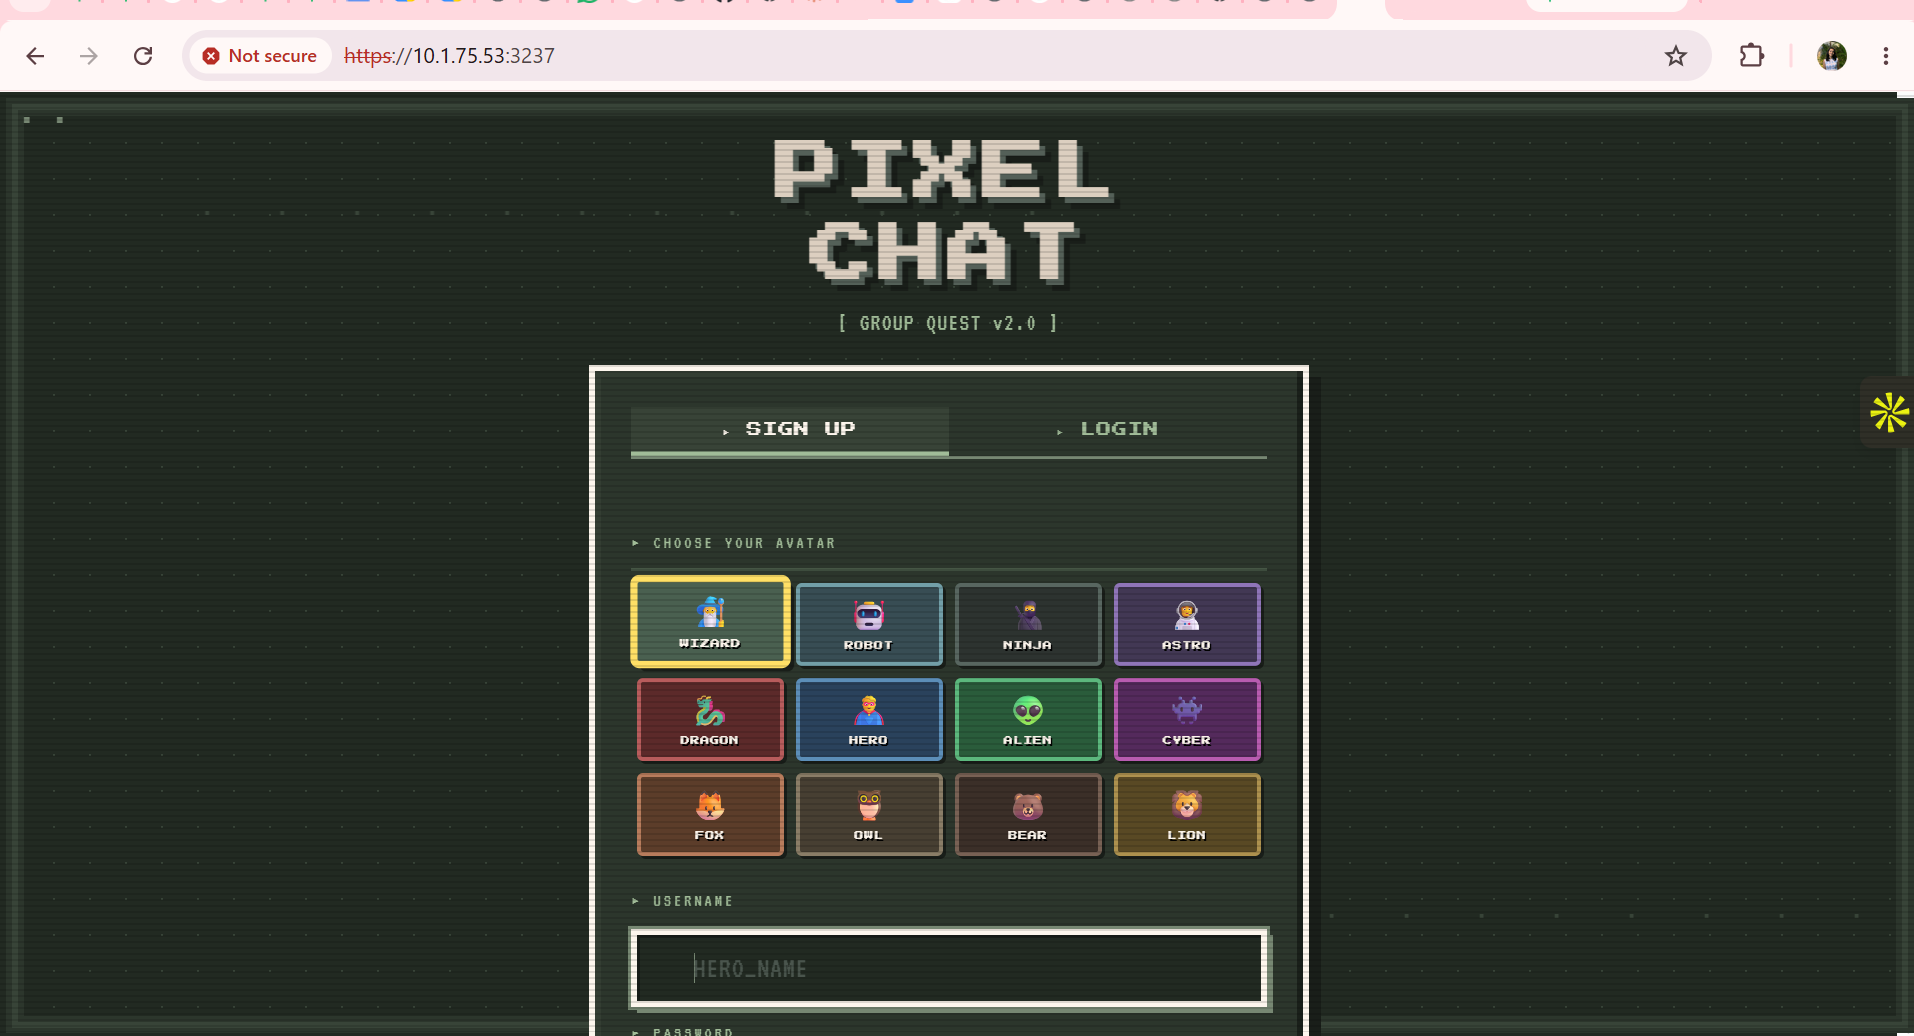
\includegraphics[width=0.85\textwidth]{p7.png}
\caption{Messaging application accessed through the load balancer}
\label{fig:messaging-integration}
\end{figure}

% ══════════════════════════════════════════════════════════════
\section{Full Load Balancer Code}
\label{sec:fullcode}

The executable entry point is \texttt{cmd/load-balancer/main.go}. The complete canonical implementation from \texttt{internal/loadbalancer/loadbalancer.go} is embedded below so this document is self-contained and compiles on Overleaf without any external Go source file.

\begin{lstlisting}[
    style=gostyle,
    basicstyle=\ttfamily\scriptsize,
    caption={Complete canonical load-balancer implementation},
    label={lst:complete-lb}
]
package loadbalancer

import (
	"bufio"
	"context"
	"crypto/tls"
	"encoding/json"
	"errors"
	"flag"
	"fmt"
	"io"
	"log"
	"net"
	"net/http"
	"net/http/httputil"
	"net/url"
	"os"
	"os/signal"
	"sort"
	"strconv"
	"strings"
	"sync"
	"sync/atomic"
	"syscall"
	"time"
)

const affinityCookieName = "pixelchat_backend"

type Backend struct {
	ID       int
	URL      *url.URL
	Alive    atomic.Bool
	InFlight atomic.Int64
}

type latencyTracker struct {
	mu         sync.Mutex
	samples    []time.Duration
	next       int
	observed   uint64
	total      time.Duration
	maxSamples int
}

func newLatencyTracker(maxSamples int) *latencyTracker {
	return &latencyTracker{maxSamples: maxSamples}
}

func (tracker *latencyTracker) observe(duration time.Duration) {
	tracker.mu.Lock()
	defer tracker.mu.Unlock()

	tracker.observed++
	tracker.total += duration
	if tracker.maxSamples == 0 {
		return
	}
	if len(tracker.samples) < tracker.maxSamples {
		tracker.samples = append(tracker.samples, duration)
		return
	}
	tracker.samples[tracker.next] = duration
	tracker.next = (tracker.next + 1) % tracker.maxSamples
}

func (tracker *latencyTracker) snapshot() map[string]any {
	tracker.mu.Lock()
	samples := append([]time.Duration(nil), tracker.samples...)
	observed := tracker.observed
	total := tracker.total
	tracker.mu.Unlock()

	sort.Slice(samples, func(i, j int) bool { return samples[i] < samples[j] })
	averageMS := 0.0
	if observed > 0 {
		averageMS = durationMS(total / time.Duration(observed))
	}
	return map[string]any{
		"count":        observed,
		"sample_count": len(samples),
		"average_ms":   averageMS,
		"p50_ms":       percentileMS(samples, 50),
		"p95_ms":       percentileMS(samples, 95),
		"p99_ms":       percentileMS(samples, 99),
	}
}

type Metrics struct {
	Total         atomic.Uint64
	Success       atomic.Uint64
	Failed        atomic.Uint64
	BackendErrors atomic.Uint64
	latencies     *latencyTracker
}

func newMetrics(maxLatencySamples int) *Metrics {
	return &Metrics{latencies: newLatencyTracker(maxLatencySamples)}
}

type LoadBalancer struct {
	backends       []*Backend
	next           atomic.Uint64
	metrics        *Metrics
	transport      *http.Transport
	healthClient   *http.Client
	backendTimeout time.Duration
	healthPath     string
	affinity       bool
	secureCookie   bool
	logger         *log.Logger
}

type config struct {
	backendsRaw               string
	port                      int
	healthInterval            time.Duration
	healthTimeout             time.Duration
	backendTimeout            time.Duration
	healthPath                string
	backendInsecureSkipVerify bool
	affinity                  bool
	tlsCert                   string
	tlsKey                    string
	maxLatencySamples         int
}

func parseBackends(raw string) ([]*Backend, error) {
	parts := strings.Split(raw, ",")
	backends := make([]*Backend, 0, len(parts))
	seen := make(map[string]struct{}, len(parts))

	for _, part := range parts {
		value := strings.TrimSpace(part)
		if value == "" {
			return nil, errors.New("backend URL list contains an empty entry")
		}
		parsed, err := url.Parse(value)
		if err != nil {
			return nil, fmt.Errorf("invalid backend URL %q: %w", value, err)
		}
		if (parsed.Scheme != "http" && parsed.Scheme != "https") || parsed.Host == "" {
			return nil, fmt.Errorf("backend URL %q must include an http or https scheme and host", value)
		}
		if parsed.User != nil {
			return nil, fmt.Errorf("backend URL %q must not contain credentials", value)
		}
		parsed.Fragment = ""
		key := parsed.String()
		if _, duplicate := seen[key]; duplicate {
			return nil, fmt.Errorf("duplicate backend URL %q", value)
		}
		seen[key] = struct{}{}

		backend := &Backend{ID: len(backends), URL: parsed}
		backend.Alive.Store(true)
		backends = append(backends, backend)
	}
	if len(backends) == 0 {
		return nil, errors.New("at least one backend URL is required")
	}
	return backends, nil
}

func (lb *LoadBalancer) nextBackend(request *http.Request) *Backend {
	if len(lb.backends) == 0 {
		return nil
	}

	if lb.affinity && request != nil {
		if cookie, err := request.Cookie(affinityCookieName); err == nil {
			if index, err := strconv.Atoi(cookie.Value); err == nil &&
				index >= 0 && index < len(lb.backends) &&
				lb.backends[index].Alive.Load() {
				return lb.backends[index]
			}
		}
	}

	// Advance past the backend that was actually selected, not merely past the
	// first candidate. This avoids repeatedly selecting the same healthy replica
	// when the candidate immediately before it is unhealthy.
	for {
		start := lb.next.Load()
		for offset := 0; offset < len(lb.backends); offset++ {
			index := (start + uint64(offset)) % uint64(len(lb.backends))
			backend := lb.backends[index]
			if backend.Alive.Load() && lb.next.CompareAndSwap(start, start+uint64(offset)+1) {
				return backend
			}
			if lb.next.Load() != start {
				break
			}
		}
		if lb.next.Load() == start {
			return nil
		}
	}
}

func (lb *LoadBalancer) backendHealthURL(backend *Backend) string {
	healthURL := *backend.URL
	healthURL.RawQuery = ""
	healthURL.Fragment = ""
	healthURL.Path = strings.TrimRight(healthURL.Path, "/") + "/" + strings.TrimLeft(lb.healthPath, "/")
	healthURL.RawPath = ""
	return healthURL.String()
}

func (lb *LoadBalancer) checkBackend(ctx context.Context, backend *Backend) {
	request, err := http.NewRequestWithContext(ctx, http.MethodGet, lb.backendHealthURL(backend), nil)
	if err != nil {
		backend.Alive.Store(false)
		return
	}
	request.Header.Set("User-Agent", "PixelChat-Load-Balancer/1.0")

	response, err := lb.healthClient.Do(request)
	healthy := err == nil && response.StatusCode == http.StatusOK
	if response != nil {
		_, _ = io.Copy(io.Discard, io.LimitReader(response.Body, 4096))
		_ = response.Body.Close()
	}
	backend.Alive.Store(healthy)
}

func (lb *LoadBalancer) checkAllBackends(ctx context.Context) {
	var waitGroup sync.WaitGroup
	for _, backend := range lb.backends {
		waitGroup.Add(1)
		go func() {
			defer waitGroup.Done()
			lb.checkBackend(ctx, backend)
		}()
	}
	waitGroup.Wait()
}

func (lb *LoadBalancer) healthLoop(ctx context.Context, interval time.Duration) {
	lb.checkAllBackends(ctx)
	ticker := time.NewTicker(interval)
	defer ticker.Stop()

	for {
		select {
		case <-ticker.C:
			lb.checkAllBackends(ctx)
		case <-ctx.Done():
			return
		}
	}
}

func (lb *LoadBalancer) statusSnapshot() map[string]any {
	statuses := make([]map[string]any, 0, len(lb.backends))
	for _, backend := range lb.backends {
		statuses = append(statuses, map[string]any{
			"url":       backend.URL.String(),
			"alive":     backend.Alive.Load(),
			"in_flight": backend.InFlight.Load(),
		})
	}
	return map[string]any{"backends": statuses}
}

func (lb *LoadBalancer) metricsSnapshot() map[string]any {
	return map[string]any{
		"total":          lb.metrics.Total.Load(),
		"success":        lb.metrics.Success.Load(),
		"failed":         lb.metrics.Failed.Load(),
		"backend_errors": lb.metrics.BackendErrors.Load(),
		"latency":        lb.metrics.latencies.snapshot(),
	}
}

func writeJSON(response http.ResponseWriter, status int, value any) {
	response.Header().Set("Content-Type", "application/json")
	response.WriteHeader(status)
	if err := json.NewEncoder(response).Encode(value); err != nil {
		log.Printf("encode JSON response: %v", err)
	}
}

func monitoringMethodAllowed(response http.ResponseWriter, request *http.Request) bool {
	if request.Method == http.MethodGet || request.Method == http.MethodHead {
		return true
	}
	response.Header().Set("Allow", "GET, HEAD")
	http.Error(response, "method not allowed", http.StatusMethodNotAllowed)
	return false
}

func (lb *LoadBalancer) handler() http.Handler {
	mux := http.NewServeMux()

	mux.HandleFunc("/lb/health", func(response http.ResponseWriter, request *http.Request) {
		if !monitoringMethodAllowed(response, request) {
			return
		}
		writeJSON(response, http.StatusOK, map[string]string{"status": "ok"})
	})
	mux.HandleFunc("/lb/status", func(response http.ResponseWriter, request *http.Request) {
		if !monitoringMethodAllowed(response, request) {
			return
		}
		writeJSON(response, http.StatusOK, lb.statusSnapshot())
	})
	mux.HandleFunc("/lb/metrics", func(response http.ResponseWriter, request *http.Request) {
		if !monitoringMethodAllowed(response, request) {
			return
		}
		writeJSON(response, http.StatusOK, lb.metricsSnapshot())
	})
	mux.HandleFunc("/", lb.proxyRequest)
	return mux
}

func (lb *LoadBalancer) proxyRequest(response http.ResponseWriter, request *http.Request) {
	start := time.Now()
	lb.metrics.Total.Add(1)

	backend := lb.nextBackend(request)
	if backend == nil {
		lb.metrics.Failed.Add(1)
		lb.metrics.latencies.observe(time.Since(start))
		http.Error(response, "no healthy backends available", http.StatusServiceUnavailable)
		return
	}

	backend.InFlight.Add(1)
	defer backend.InFlight.Add(-1)

	recorder := &statusRecorder{ResponseWriter: response}
	proxyFailed := false
	backendFailed := false
	proxy := httputil.NewSingleHostReverseProxy(backend.URL)
	proxy.Transport = lb.transport
	proxy.ErrorLog = lb.logger
	proxy.ModifyResponse = func(backendResponse *http.Response) error {
		backendResponse.Header.Set("X-Load-Balancer-Backend", backend.URL.String())
		if lb.affinity {
			backendResponse.Header.Add("Set-Cookie", (&http.Cookie{
				Name:     affinityCookieName,
				Value:    strconv.Itoa(backend.ID),
				Path:     "/",
				MaxAge:   24 * 60 * 60,
				HttpOnly: true,
				Secure:   lb.secureCookie,
				SameSite: http.SameSiteLaxMode,
			}).String())
		}
		return nil
	}
	proxy.ErrorHandler = func(proxyResponse http.ResponseWriter, proxyRequest *http.Request, err error) {
		proxyFailed = true
		// A downstream client that times out or disconnects cancels the original
		// request context. That does not prove the selected backend is unhealthy,
		// so keep it in rotation. Proxy/backend timeouts occur while the original
		// client context is still live and continue to eject the backend.
		backendFailed = request.Context().Err() == nil
		if backendFailed {
			backend.Alive.Store(false)
		}
		if !recorder.wroteHeader {
			http.Error(proxyResponse, "backend unavailable", http.StatusBadGateway)
		}
	}

	proxyRequest := request
	cancel := func() {}
	if !isUpgradeRequest(request) {
		var contextWithTimeout context.Context
		contextWithTimeout, cancel = context.WithTimeout(request.Context(), lb.backendTimeout)
		proxyRequest = request.WithContext(contextWithTimeout)
	}
	defer cancel()

	proxy.ServeHTTP(recorder, proxyRequest)

	lb.metrics.latencies.observe(time.Since(start))
	status := recorder.status()
	if proxyFailed {
		lb.metrics.Failed.Add(1)
		if backendFailed {
			lb.metrics.BackendErrors.Add(1)
		}
		return
	}
	if status >= 100 && status < 400 {
		lb.metrics.Success.Add(1)
		return
	}
	lb.metrics.Failed.Add(1)
	if status >= 500 {
		lb.metrics.BackendErrors.Add(1)
	}
}

func isUpgradeRequest(request *http.Request) bool {
	if strings.TrimSpace(request.Header.Get("Upgrade")) == "" {
		return false
	}
	for _, token := range strings.Split(request.Header.Get("Connection"), ",") {
		if strings.EqualFold(strings.TrimSpace(token), "upgrade") {
			return true
		}
	}
	return false
}

type statusRecorder struct {
	http.ResponseWriter
	statusCode  int
	wroteHeader bool
}

func (recorder *statusRecorder) Unwrap() http.ResponseWriter {
	return recorder.ResponseWriter
}

func (recorder *statusRecorder) status() int {
	if recorder.statusCode == 0 {
		return http.StatusOK
	}
	return recorder.statusCode
}

func (recorder *statusRecorder) WriteHeader(statusCode int) {
	if recorder.wroteHeader {
		return
	}
	recorder.statusCode = statusCode
	recorder.wroteHeader = true
	recorder.ResponseWriter.WriteHeader(statusCode)
}

func (recorder *statusRecorder) Write(payload []byte) (int, error) {
	if !recorder.wroteHeader {
		recorder.WriteHeader(http.StatusOK)
	}
	return recorder.ResponseWriter.Write(payload)
}

func (recorder *statusRecorder) Flush() {
	if !recorder.wroteHeader {
		recorder.WriteHeader(http.StatusOK)
	}
	if flusher, ok := recorder.ResponseWriter.(http.Flusher); ok {
		flusher.Flush()
	}
}

func (recorder *statusRecorder) Hijack() (net.Conn, *bufio.ReadWriter, error) {
	hijacker, ok := recorder.ResponseWriter.(http.Hijacker)
	if !ok {
		return nil, nil, errors.New("underlying response writer does not support hijacking")
	}
	return hijacker.Hijack()
}

func (recorder *statusRecorder) Push(target string, options *http.PushOptions) error {
	if pusher, ok := recorder.ResponseWriter.(http.Pusher); ok {
		return pusher.Push(target, options)
	}
	return http.ErrNotSupported
}

func (recorder *statusRecorder) ReadFrom(source io.Reader) (int64, error) {
	if !recorder.wroteHeader {
		recorder.WriteHeader(http.StatusOK)
	}
	if readerFrom, ok := recorder.ResponseWriter.(io.ReaderFrom); ok {
		return readerFrom.ReadFrom(source)
	}
	return io.Copy(recorder.ResponseWriter, source)
}

func percentileMS(sortedDurations []time.Duration, percentile int) float64 {
	if len(sortedDurations) == 0 {
		return 0
	}
	index := (percentile*len(sortedDurations) + 99) / 100
	index = max(1, min(index, len(sortedDurations)))
	return durationMS(sortedDurations[index-1])
}

func durationMS(duration time.Duration) float64 {
	return float64(duration) / float64(time.Millisecond)
}

func validateConfig(configuration config) error {
	if strings.TrimSpace(configuration.backendsRaw) == "" {
		return errors.New("provide backend URLs using -backends")
	}
	if configuration.port < 1 || configuration.port > 65535 {
		return errors.New("-port must be between 1 and 65535")
	}
	if configuration.healthInterval <= 0 {
		return errors.New("-health-interval must be greater than zero")
	}
	if configuration.healthTimeout <= 0 {
		return errors.New("-health-timeout must be greater than zero")
	}
	if configuration.backendTimeout <= 0 {
		return errors.New("-backend-timeout must be greater than zero")
	}
	if strings.TrimSpace(configuration.healthPath) == "" {
		return errors.New("-health-path must not be empty")
	}
	if configuration.maxLatencySamples < 0 {
		return errors.New("-max-latency-samples must not be negative")
	}
	if (configuration.tlsCert == "") != (configuration.tlsKey == "") {
		return errors.New("-tls-cert and -tls-key must be provided together")
	}
	return nil
}

func newLoadBalancer(configuration config, backends []*Backend, logger *log.Logger) *LoadBalancer {
	tlsConfiguration := &tls.Config{
		MinVersion:         tls.VersionTLS12,
		InsecureSkipVerify: configuration.backendInsecureSkipVerify,
	}
	transport := &http.Transport{
		Proxy:                 http.ProxyFromEnvironment,
		DialContext:           (&net.Dialer{Timeout: 2 * time.Second, KeepAlive: 30 * time.Second}).DialContext,
		ForceAttemptHTTP2:     true,
		MaxIdleConns:          256,
		MaxIdleConnsPerHost:   128,
		IdleConnTimeout:       90 * time.Second,
		TLSHandshakeTimeout:   2 * time.Second,
		ResponseHeaderTimeout: configuration.backendTimeout,
		TLSClientConfig:       tlsConfiguration,
	}
	healthTransport := transport.Clone()
	healthTransport.MaxIdleConnsPerHost = 4

	return &LoadBalancer{
		backends:       backends,
		metrics:        newMetrics(configuration.maxLatencySamples),
		transport:      transport,
		healthClient:   &http.Client{Transport: healthTransport, Timeout: configuration.healthTimeout},
		backendTimeout: configuration.backendTimeout,
		healthPath:     configuration.healthPath,
		affinity:       configuration.affinity,
		secureCookie:   configuration.tlsCert != "",
		logger:         logger,
	}
}

func RunCLI(arguments []string, standardOutput io.Writer, standardError io.Writer) int {
	flags := flag.NewFlagSet("load-balancer", flag.ContinueOnError)
	flags.SetOutput(standardError)

	configuration := config{}
	flags.StringVar(&configuration.backendsRaw, "backends", "", "Comma-separated backend URLs")
	flags.IntVar(&configuration.port, "port", 8080, "Load balancer listen port")
	flags.DurationVar(&configuration.healthInterval, "health-interval", time.Second, "Health check interval")
	flags.DurationVar(&configuration.healthTimeout, "health-timeout", 2*time.Second, "Per-backend health check timeout")
	flags.DurationVar(&configuration.backendTimeout, "backend-timeout", 3*time.Second, "Total timeout for non-upgraded backend requests")
	flags.StringVar(&configuration.healthPath, "health-path", "/health", "Backend health check path")
	flags.BoolVar(&configuration.backendInsecureSkipVerify, "backend-insecure-skip-verify", false, "Accept self-signed backend TLS certificates (lab only)")
	flags.BoolVar(&configuration.affinity, "affinity", true, "Enable browser cookie affinity for stateful messaging sessions")
	flags.StringVar(&configuration.tlsCert, "tls-cert", "", "PEM certificate for HTTPS listener")
	flags.StringVar(&configuration.tlsKey, "tls-key", "", "PEM private key for HTTPS listener")
	flags.IntVar(&configuration.maxLatencySamples, "max-latency-samples", 100000, "Maximum recent latency samples kept for percentiles (0 disables samples)")

	if err := flags.Parse(arguments); err != nil {
		if errors.Is(err, flag.ErrHelp) {
			return 0
		}
		return 2
	}
	if err := validateConfig(configuration); err != nil {
		fmt.Fprintf(standardError, "load-balancer: %v\n", err)
		return 2
	}
	backends, err := parseBackends(configuration.backendsRaw)
	if err != nil {
		fmt.Fprintf(standardError, "load-balancer: %v\n", err)
		return 2
	}

	logger := log.New(standardError, "load-balancer: ", log.LstdFlags)
	balancer := newLoadBalancer(configuration, backends, logger)
	server := &http.Server{
		Addr:              fmt.Sprintf(":%d", configuration.port),
		Handler:           balancer.handler(),
		ReadHeaderTimeout: 5 * time.Second,
		IdleTimeout:       120 * time.Second,
	}

	ctx, stop := signal.NotifyContext(context.Background(), os.Interrupt, syscall.SIGTERM)
	defer stop()
	balancer.checkAllBackends(ctx)
	go balancer.healthLoop(ctx, configuration.healthInterval)

	scheme := "http"
	if configuration.tlsCert != "" {
		scheme = "https"
	}
	fmt.Fprintf(standardOutput, "Load balancer listening on %s://localhost:%d with %d backend(s)\n", scheme, configuration.port, len(backends))

	errorChannel := make(chan error, 1)
	go func() {
		if configuration.tlsCert != "" {
			errorChannel <- server.ListenAndServeTLS(configuration.tlsCert, configuration.tlsKey)
			return
		}
		errorChannel <- server.ListenAndServe()
	}()

	select {
	case serveError := <-errorChannel:
		if serveError != nil && !errors.Is(serveError, http.ErrServerClosed) {
			logger.Printf("server failed: %v", serveError)
			return 1
		}
	case <-ctx.Done():
		shutdownContext, cancel := context.WithTimeout(context.Background(), 5*time.Second)
		defer cancel()
		if err := server.Shutdown(shutdownContext); err != nil {
			logger.Printf("graceful shutdown failed: %v", err)
			return 1
		}
	}
	return 0
}
\end{lstlisting}

% ══════════════════════════════════════════════════════════════
\section{Conclusion}

This lab successfully demonstrated the design, implementation, and evaluation of a load-balanced back-end system. Key accomplishments:

\begin{enumerate}[leftmargin=2em]
    \item Implemented a fully functional \textbf{Go reverse-proxy load balancer} with round-robin scheduling, health checking, configurable timeouts, and monitoring endpoints.
    \item Deployed the \textbf{messaging application back-end} across three machines (Sys2, Sys3, Sys4).
    \item Built a \textbf{concurrent load generator} that measures throughput, dropout, and latency percentiles.
    \item Conducted controlled experiments comparing single vs.\ three backend performance.
    \item The controlled local-workstation run measured \textbf{29.5\% higher throughput}, \textbf{27.9\% lower p50 latency}, and \textbf{35.9\% lower p95 latency} with three backends. One of 5,000 three-backend requests timed out and p99 was 14.8\% higher; both limitations are reported transparently.
\end{enumerate}

\end{document}
